\input{include}
\usepackage{multirow}
\AtBeginBibliography{\tiny}

\title{music informatics group}
\subtitle{overview} 

%%%%%%%%%%%%%%%%%%%%%%%%%%%%%%%%%%%%%%%%%%%%%%%%%%%%%%%%%%%%%%%%%%%%%%%%%%%%
\begin{document}
    % generate title page
	\input{include/titlepage}

    \section[about]{about music informatics group}
        %\input{dolby}
        %\begin{frame}{about}{self-introduction}
    %\begin{itemize}
        %\item   \textbf{education}
            %\begin{itemize}
                %\item   Electrical Engineering (Technical University Berlin)
                %\item   Tonmeister (music production, University of Arts Berlin)
            %\end{itemize}
        %\bigskip
        %\item   \textbf{professional}
            %\begin{itemize}
                %\item   Associate Professor at the \href{https://music.gatech.edu}{School of Music, Georgia Institute of Technology}
                %\item   2000-2013: Head of Research at \href{https://www.zplane.de}{zplane.development}
            %\end{itemize}
        %\bigskip
        %\item   \textbf{background}
            %\begin{itemize}
                %\item   audio algorithm design (20+ years)
                %%\item   classical musician (20+ years)
                %\item   commercial music software development (10+ years)
                %\item   entrepreneurship (10+ years)
            %\end{itemize}
    %\end{itemize}
    %
    %\addreference{\href{https://www.linkedin.com/in/lerch}{www.linkedin.com/in/lerch}}
    %%\inserticon{person}
    %\vspace{-30mm}
    %\begin{flushright}
                            %\includegraphics[scale=.20]{cover_aca2_thumb}
    %\end{flushright}
%
%\end{frame}

\begin{frame}{introduction}{music informatics group}
    \vspace{-5mm}
    \begin{columns}
    \column{.6\linewidth}
    \begin{itemize}
        %\item   \textbf{research focus}
            %\begin{itemize}
                %\item   machine learning and intelligent DSP solutions for (musical) audio 
            %\end{itemize}
        %\bigskip
        \item   \textbf{mission}
            \begin{itemize}
                \item   create new technologies transforming and improving how we \textit{make, produce, perform, discover, and consume music}
                \item   advance the field of AI for audio through \textit{knowledge-driven machine learning}
            \end{itemize}
        \bigskip
        \item   \textbf{objectives}
            \begin{itemize}
                \item   enable/improve \textit{machine understanding of music} and musical language
                \item   create \textit{interpretable and controllable systems}
                \item   design algorithms with \textit{low data requirements}
            \end{itemize}
    \end{itemize}
    \column{.4\linewidth}
        \vspace{12mm}
        \begin{figure}%
            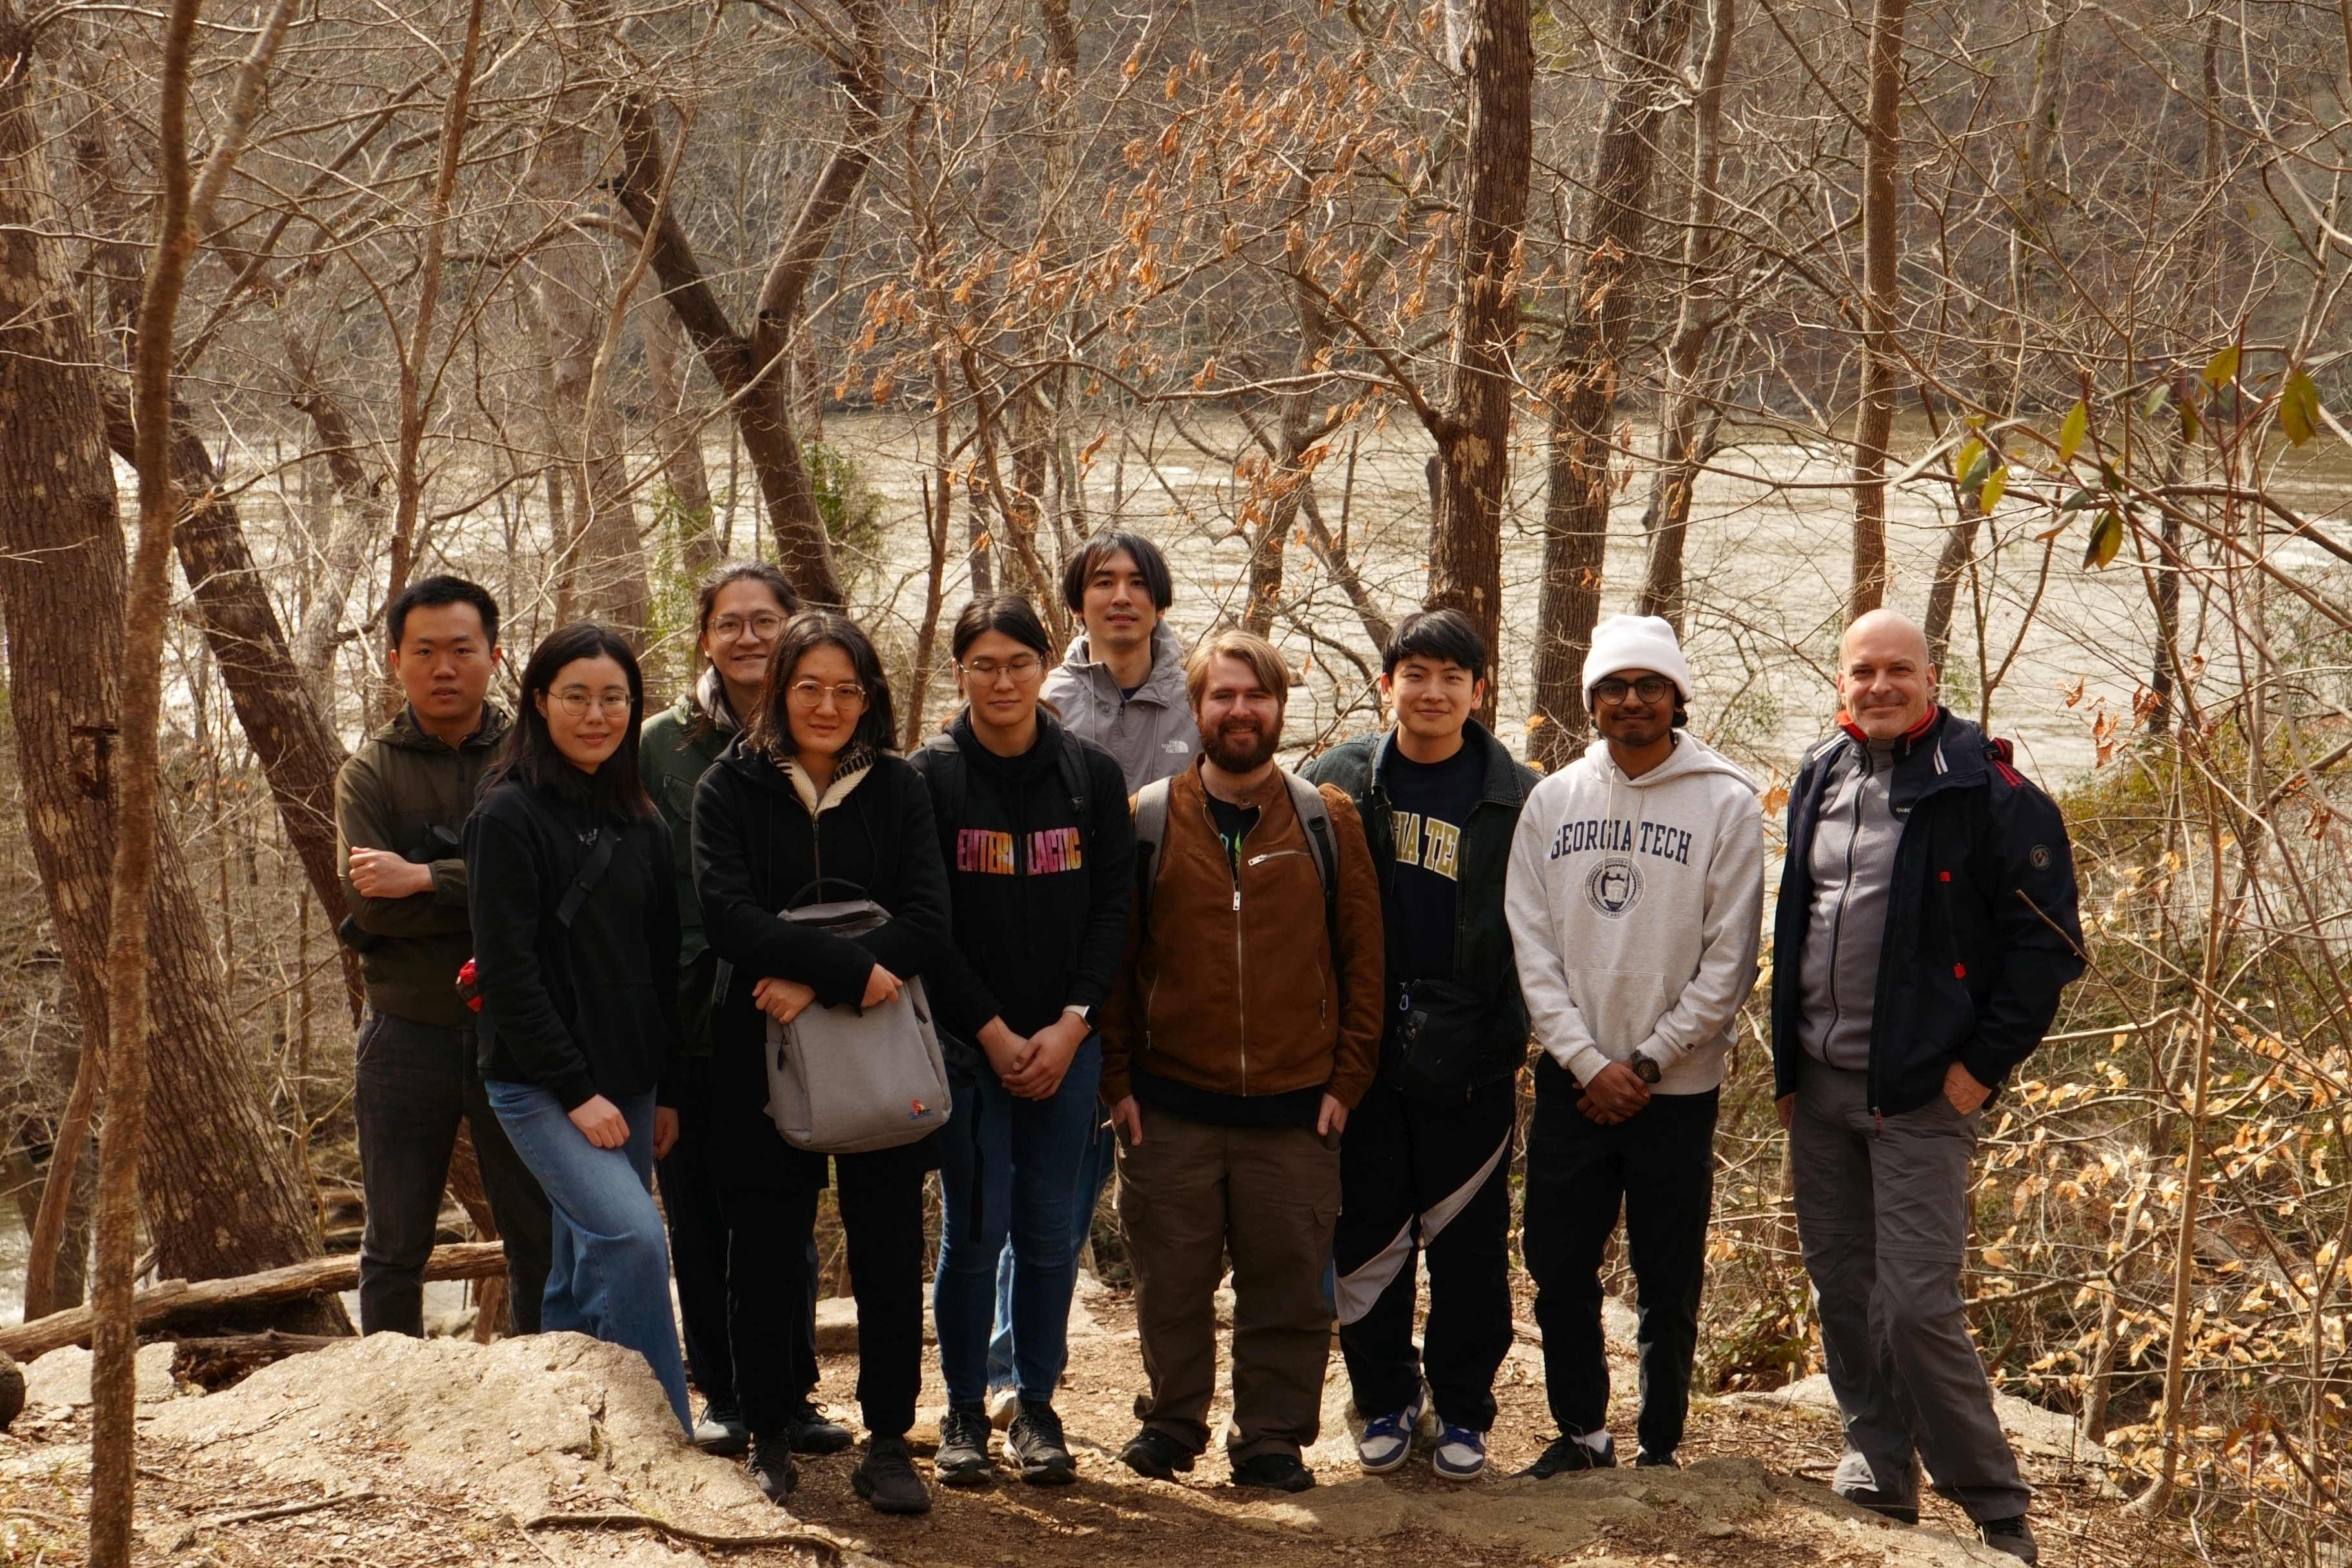
\includegraphics[width=\columnwidth]{MIG2025}%
        \end{figure}
    \end{columns}
    {\addreference{\href{https://musicinformatics.gatech.edu}{musicinformatics.gatech.edu}}}
    %\inserticon{person}
\end{frame}

        
    \section[areas]{areas}
        \begin{frame}{tasks}{selected tasks of interest}
            \vspace{-9mm}
            \begin{columns}
            \column{.6\linewidth}
            \begin{itemize}
                \item   \textbf{audio content analysis} \cite{lerch_introduction_2023}
                    \begin{itemize}
                        \item   music/audio \textit{classification}
                            \begin{itemize}
                                \item genre/events \cite{burred_hierarchical_2004, hung_low-resource_2023}
                                \item instruments \cite{gururani_semi-supervised_2021, chen_music_2023, ding_audio_2023}
                                \item tagging \cite{ding_audio_2023, ding_embedding_2024, ma_music_2024}
                                \item emotion \cite{watcharasupat_uncertainty_2025}
                                \item pedestrians \cite{seshadri_asped_2024, han_understanding_2024}
                            \end{itemize}
                        \item   music \textit{transcription}
                            \begin{itemize}
                                \item drum transcription \cite{wu_review_2018}
                                \item chord detection \cite{zhou_chord_2015}
                            \end{itemize}
                        \item   music \textit{performance analysis} \cite{pati_assessment_2018}
                    \end{itemize}
                 \smallskip
                 \item<2->  \textbf{music source separation} \cite{hung_multi-task_2020, watcharasupat_generalized_2024, watcharasupat_stem-agnostic_2024}
                 \smallskip
                 \item<3->  \textbf{sound and music generation}
                    \begin{itemize}
                        \item   controllability \cite{pati_attribute-based_2020}
                        \item   evaluation \cite{yang_evaluation_2020, pati_is_2021, watcharasupat_latte_2022, vinay_evaluating_2022}
                    \end{itemize}
            \end{itemize}
            \column{.4\linewidth}
            \begin{figure}
                \includegraphics[scale=.20]{cover_aca2_thumb}
            \end{figure}
            \end{columns}
            \vspace{-25mm}
            \begin{flushright}
                \includegraphics[scale=.25]{forensics}
            \end{flushright}
        \end{frame}
        
     \section[methods]{methods}
        \begin{frame}{methods}{methods of interest}
            \begin{itemize}
                \item   \textbf{knowledge transfer \& representation learning}
                    \begin{itemize}
                        \item   improved structure of embedded representations \cite{seshadri_improving_2021, ma_representation_2022}
                        \item   enforcing the meaning of specific embedding dimensions \cite{pati_attribute-based_2020, pati_is_2021}
                        \item   knowledge transfer \cite{hung_feature-informed_2022, ding_audio_2023, ding_embedding_2024}
                    \end{itemize}
                 \bigskip
                 \item<2->  \textbf{low-resource machine learning}
                    \begin{itemize}
                        \item   semi- and self-supervised learning \cite{gururani_semi-supervised_2021, wu_labeled_2018}
                        \item   reprogramming \cite{chen_music_2023, hung_low-resource_2023}
                    \end{itemize}
                 \bigskip
                 \item<3->  \textbf{objective evaluation of generative systems}
                    \begin{itemize}
                        \item   evaluation of controllable systems with correlated attributes \cite{watcharasupat_evaluation_2021, watcharasupat_latte_2022}
                        \item   statistical models for comparison of properties \cite{yang_evaluation_2020}
                        \item   metrics for sound generation \cite{vinay_evaluating_2022}
                    \end{itemize}
            \end{itemize}
            \vspace{-40mm}
            \begin{flushright}
                \includegraphics[scale=.20]{machinelearning}
            \end{flushright}
            \end{frame}
        
        \section[links]{thank you}

      \begin{frame}\frametitle{links}\framesubtitle{~}
            %\addreference{\href{https://github.com/alexanderlerch}{github.com/alexanderlerch}}
            \begin{block}{links}
                music informatics group:
                \href{http://musicinformatics.gatech.edu}{musicinformatics.gatech.edu}

                \bigskip
                alexander lerch: 
                    \begin{itemize}
                        \item \href{https://www.linkedin.com/in/lerch}{www.linkedin.com/in/lerch}
                        \item \href{https://github.com/alexanderlerch}{github.com/alexanderlerch}
                        \item mail: \href{mailto:alexander.lerch@gatech.edu}{alexander.lerch@gatech.edu}
                    \end{itemize}             
                %\href{http://www.alexanderlerch.com}{www.alexanderlerch.com}
                
                \bigskip                
                book: \href{https://www.AudioContentAnalysis.org}{www.AudioContentAnalysis.org}
                
                %\visible<1->{
								%\vspace{-25mm}
                %\begin{flushright}
										%\includegraphics[scale=.20]{cover_aca2_thumb}
                %\end{flushright}
                %\vspace{-15mm}}

								%\pause
                %\bigskip
                %zplane.development: 
                %\href{https://www.zplane.de}{www.zplane.de}

                %\pause
								
								\vspace{5mm}

            \end{block}
            
			%\vspace{-22mm}
						\inserticon{mail}
            %\includegraphics[scale=.1]{wechat_qr}%
            %\begin{textblock*}{110mm}(14.25cm,7.3cm)
                %\includegraphics[height=1.25cm,keepaspectratio]{mail}
            %\end{textblock*}            
        \end{frame}

    
    \begin{frame}[allowframebreaks]{references}{references}
    \tiny
        \printbibliography
    \end{frame}
\end{document}

